\subsubsubsubsection{Urban entity}
\begin{figure}[h]
\centering
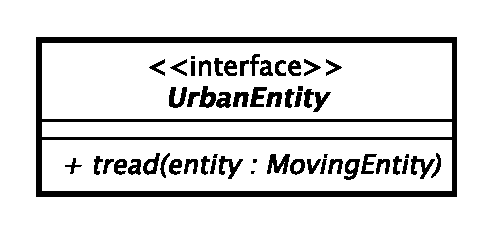
\includegraphics[scale=0.6,keepaspectratio]{images/solution/app/backend/urban_entity.eps}
\caption{\pReactiveComponent::UrbanEntity}
\label{fig:sd-app-urban-entity}
\end{figure}
\FloatBarrier
\begin{itemize}
  \item \textbf{\descr} \\
    It represents one of the entities the district infrastructure is composed
    of.
  \item \textbf{\ops}
  \begin{itemize} 
    \item[+] \texttt{\textit{tread(entity: MovingEntity)}} \\
    Abstract method through which the urban infrastructure can be treaded by a
    moving entity.
  \end{itemize}
\end{itemize}
